\definecolor{codegreen}{rgb}{0,0.6,0}
\lstdefinestyle{mystyle}{
    keywordstyle=\color{magenta},
    commentstyle=\color{codegreen},
    language=Java,
    basicstyle=\ttfamily\footnotesize,
    breakatwhitespace=true,         
    breaklines=true,                 
    captionpos=b,                    
    keepspaces=true,                 
    numbers=left,                    
    numbersep=5pt,                  
    showspaces=false,                
    showstringspaces=false,
    showtabs=false,                  
    tabsize=2
}
\lstset{style=mystyle}


\chapter{Implementation}
\label{ch:implementation}
The project has been implemented in 3 stages, similar to the 3 sections of our design. These are: The Emulator described in Chapter \ref{sec:impl_emul}, Visualisation in Chapter \ref{sec:impl_vis} and the Module System in Chapter \ref{sec:impl_mod}. 

The module system was a later addition to the project, hence its separate design and implementation sections, instead of being directly implemented from the beginning, its respective changes and alterations to the implementation are discussed in its respective section.

First a few bits of terminology should be covered:

\begin{itemize}
    \item \textbf{Instance} - An instance is a physical manifestation of a class during runtime. It can be physically interacted with, providing the written functionality.
    \item \textbf{Abstract Class} - An abstract class is a class that cannot be directly instantiated. It provides a set of implemented and unimplemented methods (labelled abstract). The abstract class must be extended, with any abstract methods implemented.
    \item \textbf{Interface} - An interface is an abstract type that declares behaviour a class must implement, containing a set of method and constant declarations that any implementing class must implement.
\end{itemize}

\section{Emulator}\label{sec:impl_emul}
At its base the emulator provides implementations of the core components to emulate RISC-V instructions. These are representations of physical register, memory and instructions. These three allow us to completely emulate any RISC-V instruction. A further part of the emulator is the parser, which provides essentially functionality to covert user written programs into a representation the emulator can understand.

Below, each of the 3 core components is discussed as well as the other relevant details allowing for the complete implementation of the emulator.

\subsection{Binary Class}
Originally the emulator stored the respective binary values of register and memory values as a integer, due to the fact that RISC-V deals with 32 it twos-compliment numbers, and Java's integer is also 32 bit twos-compliment. Whilst some instructions suited this making use of just basic arithmetic operations, it was quickly noted that instructions started to operate on the binary form.

It was decided to switch to a more intuitive representation as noted in our design in Figure \ref{fig:bin_regmem_uml}, by creating a custom \texttt{Binary} class. This class holds a string representing the 32 ones and zeros making up the value, which can then be retrieved as denary, hex or the binary value itself.

Further, additional methods could be provided directly on the \texttt{Binary} class, including the ability to sign extends values, get a certain amount of bits and also directly retrieve a new instance directly from an integer value as seen in Listing \ref{lst:binary}.

\begin{lstlisting}[caption=Additional Binary Methods, label=lst:binary]
public class Binary {
    ...
    public Binary getBits(int bits) {
        return new Binary(this.value.substring(this.value.length()-bits, this.value.length()));
    }

    public Binary getBitsSignExtended(int bits){
        Binary b = new Binary("0");
        b.setSignExtendedValue(this.value.substring(this.value.length()-bits, this.value.length()));
        return b;
    }

    public static Binary of(int value) {
        return new Binary(Integer.toBinaryString(value));
    }
}
\end{lstlisting}

As a result of switching from storing value as a integer to using this \texttt{Binary} class, it streamlined our implementation and provided a consistent way to manage binary values between the registers, memory and instructions whilst avoiding large amounts of conversion to and from integers.

\subsection{Registers}
Being the most core element of RISC-V, registers we the first component to be implemented. As per our design, each Register is represented as a instance of the \texttt{Register} class. As seen in Listing \ref{lst:register}, each register stores its name and alternate application binary interface name under the \texttt{name} and \texttt{nick} fields respectively, as well as a reference to its \texttt{Binary} instance storing the registers actual value.

\begin{lstlisting}[caption=Register Implementation, label=lst:register]
public class Register {
    private final String name, nick;

    private Binary binary;

    public Register(String name, String nick) {
        this.name = name;
        this.nick = nick;

        this.binary = new Binary("0");
    }

    // EXCLUDING ALL GET/SET METHODS 
    ...

    public void reset() {
        this.setValue("0");
    }
    public Register clone(){
        Register rnew = new Register(this.name, this.nick);
        rnew.setValue(this.getBinary());
        return rnew;
    }
}
\end{lstlisting}

The class also provides a host of methods to get the registers value, either directly returning the \texttt{Binary} instance via \texttt{getBinary} or returning representations of the value via the respective \texttt{getValueAs...()} method, which in turn calls the respective method on the \texttt{Binary} instance.

To represent the 32 base registers a mapping of each registers name and nickname is stored to the individual register. In order to conveniently store and access all these register a manager class called \texttt{RegisterSet} is used. An instance can be created specifying how many registers, a prefix, and a list of alternate names for each register, allowing it to be re-used for more than just the 32 base registers. This functionality cannot reside in the \texttt{Register} class itself since it would all have to exist in a static context which would violate object oriented programming principles \cite{wegner_1990_concepts}. It also avoids confusing the usage of \texttt{Register}'s as actual registers and also a management interface for retrieving and storing different registers concurrently.

For the specified amount of registers, a new instance of the \texttt{Register} class is created, and is added to a map data structure directly linking each register to its respective name, and optionally its alternate application binary interface name. This can be seen in Listing \ref{lst:reg_set}.

\begin{lstlisting}[caption=RegisterSet generation, label=lst:reg_set]
 public RegisterSet(String registerPrefix, int amount, List<String> registerNicks) {
    this.prefix = registerPrefix;
    this.registerMap = new HashMap<>();

    for (int i = 0; i < amount; i++) {
        String name = registerPrefix + i;
        String nick = registerNicks != null ? registerNicks.get(i) : null;
        Register register = new Register(registerPrefix + i, nick == null ? "" : nick);
        registerMap.put(name, register);
        if (nick != null) registerMap.put(nick, register);
    }

    RegisterSet.all.add(this);
}
\end{lstlisting}

This newly created instance of \texttt{RegisterSet} allows us to now interface with each register when needed. A individual register can be requested by specifying its name. The \texttt{RegisterSet} provides methods to directly read and write the integer or binary representation as a string/hex/integer value. Alternatively, a \texttt{Register} can be directly loaded and its instance used.

Within the write method, overloading is used to allow the same method to be called with different parameter types, which internally covert the data type and call the main write method, which locates and updated the respective register. Overloading works by allowing multiple methods share the same name, but expect different parameter types. Listing \ref{lst:write_overloading} demonstrating the write implementation with a base \texttt{write} method expecting a register name and binary string, and then two overloading methods taking in an Integer and Hex string respectively, converting it to a binary string and passing to our base method.

\begin{lstlisting}[caption=Write overloading, label=lst:write_overloading]
public void writeHex(String registerName, String hexValue) throws RegisterNotFoundException, InvalidValueException {
    int intHex = Utils.formattedHexToInt(hexValue);
    this.write(registerName, Integer.toBinaryString(intHex));
}

public void writeInt(String registerName, int intValue) throws RegisterNotFoundException, InvalidValueException {
    this.write(registerName, Integer.toBinaryString(intValue));
}

public void write(String registerName, String value) throws RegisterNotFoundException, InvalidValueException {
    if (ignoreZeroRegister(registerName)) return;

    // Check the given value is infact binary
    Utils.isBinary(value); // throws its own error

    if (!SettingsController.areAnimationsEnabled()) {
        Register reg = this.load(registerName);
        reg.setValue(value);
        return;
    }

    Register cloned = this.load(registerName).clone();
    cloned.setValue(value);
    this.toUpdate.add(cloned);
}
\end{lstlisting}

It is important to note that a new \texttt{Register} instance is created here and called to be updated. This originally wasn't the case and was directly updated in the map. However this change was made to improve visualisation performance, and it will be discussed further when exploring how the emulation and visualisation is integrated as seen in Section \ref{sec:impl_integ}.

A specific case is checked for registers. As per the RISC-V specification \cite{riscv_2015_riscv}, register \verb|x0| should not be writable, and remain a constant 0. Thus, we make a check for a write to this register, ignoring any that occur. This could pose an issue due to our reusable nature of the \texttt{RegisterSet} class. However, all of the extensions for RISC-V call for a constant 0 register, and if a new one should stray from this format, it is feasible to implement a check for if writing to 0 should be allowed or not.

\subsection{Memory}
\texttt{Memory} operates similarly to registers. However, memory is created on-demand as to not waste \ac{UI} and physical memory space as often values remain empty. The memory is also 4 byte aligned, rather than specifically addressed via apre-assigned name.

Each value in memory exists as an instance of the \texttt{MemoryValue} class. This class is a near carbon copy of the \texttt{Register} class in Listing \ref{lst:register}, with references to names removed, in turn of a reference to its location in memory. It may of been ideal to have both implement an interface representing the common methods. However due to their completely independent uses, this use of inheritance would of provided little functional benefit.

\texttt{MemoryValue}'s are stored in a map, with the map mapping integer locations to each \texttt{MemoryValue} inside a \texttt{Memory} instance. Unlike the \texttt{RegisterSet} class, the \texttt{Memory} class is not reusable. This choice was made for simplicity, and following the design of RISC-V, in which only one memory exists for data. 

As states earlier, each \texttt{MemoryValue} is only created when required. This is achieved through a \texttt{load(...)} method in Listing \ref{lst:mem_load} which makes use of the maps \texttt{computeIfAbsent} method. This returns the respective \texttt{MemoryValue} for the given location. Otherwise, a new instance is created and stored against the requested location in the map and also returned avoiding an additional \texttt{get()} call. This way allows us to avoid having to perform a check to see if the location has a value each time, and then create a new instance ourselves, leaving this functionality to the builtin method.

\begin{lstlisting}[caption=Memory load method, label=lst:mem_load]
public MemoryValue load(MemoryAddress address) throws InvalidValueException, RegisterNotFoundException, InvalidMemoryAddressException {
    return this.memoryMap.computeIfAbsent(address.getAddress(), x -> {
        MemoryValue mv = null;
        try {
            mv = new MemoryValue("00000000000000000000000000000000", address.getAddress());
        } catch (Exception e) {
            //
        }
        if (newValueBind != null) newValueBind.execute(mv); return mv;});
}
\end{lstlisting}

In the \texttt{load} method we chose to do nothing with an exception raised from an invalid address as a result of \texttt{address.getAddress()} as all calls to load should be after a call to the \texttt{checkAddress} method. This method firstly checks if the address is an the valid format, returning the integer address or throwing an \texttt{InvalidMemoryAddressException}, then checking it is aligned by taking modulo 4 of the address, throwing a \texttt{UnalignedMemoryAccessException} if not aligned, with the method returning nothing for a successful address, or throwing one of the exceptions for an invalid address.

The use of this slightly sophisticated memory address checking is required due to RISC-V's specification of memory addressing in the form of \verb|offset(register)| in which the given offset may be either a denary value, or a hexadecimal value. Each of which must specifically parsed, and checked, along with the actual register being checked to ensure it exists, as this format is not specific to the base 32 bit implementation. 

The exact implementation of the memory address parsing will be discussed further in the Parser section (\ref{sec:impl_parser}).

\subsection{Singleton vs Dependency Injection}
Within our register and memory implementation, both must be easily accessible to the rest of the program, especially instructions. There are two methods to achieving this: Singleton and Dependency Injection.

\subsubsection{Singleton}
The Singleton pattern is a \textbf{Creational Pattern} allows us to ensure that only a singular instance of a class exists. It provides global access to this instance, creating it on the first access, storing it and returning this same stored instance every time. Listing \ref{lst:singleton} shows an example of this as used with the \texttt{Memory} implementation, which can be obtained using \verb|Memeory.getMemory()|.

\begin{lstlisting}[caption=Singleton pattern using within the \texttt{Memory} class, label=lst:singleton]
private static Memory memory;

public static Memory getMemory() {
    if (memory == null) {
        memory = new Memory();
    }
    return memory;
}
\end{lstlisting}

This pattern however does provide an issue. It promotes the use of static allowing easy access to the instance without having to pass around a reference to the class. Unfortunately, for novice developers this often leads to the abuse of static to make variables accessible globally for ease of use, with this commonly being referred to as "static abuse" \cite{zivkovic_2021_3}, resulting in a deviation away from object oriented programming.

However, this pattern was chosen based on reducing deeply nesting dependency injection and providing a singular instance of Registers and Memory, making it difficult to accidentally create another.

\subsubsection{Dependency Injection}
On the other hand, Dependency Injection is a \textbf{Design Pattern}. Working via the method of passing a given instance through function parameters such it may then be used. Dependency Injection doesn't determine how many instances may exists, but still provides the ability to make any instance available when needed.

An example of Dependency Injection can be seen when the optional nickname list is passed into the \texttt{RegisterSet} class in Listing
\ref{lst:reg_set}. In this case an instance of a List is provided.

Dependency Injection is useful for passing around any instance of a class, but can become convoluted when a instance is required far down a function tree, which results in parameter drilling, with many methods having the provide the instance as a parameter, to pass it down to the method that needs it, which is often resolved by refactoring large chunks of code, or by switching to a singleton pattern when possible.

\subsection{Instructions}
The implementation of the instructions follows the design as outlined in Section \ref{sec:parser}, with an abstract \texttt{Instruction} class containing the base logic for every instruction. 

The \texttt{Instruction} class holds a reference to the registers and memory, as well as providing an \texttt{execute()} method that is abstract. Such that each extending class must implement it, allowing each implementation to provide its respective instruction logic. The \texttt{Instruction} class also specifies for a list of parsible types to be provided, which correspond to the respective instruction format and its expected inputs which will be discussed further in Section \ref{sec:impl_parser}.

\begin{lstlisting}[caption=Implemented ADDI Insstruction, label=lst:addi]
public class ADDI extends Instruction {

    public ADDI() {
        // Parameter types are specifeid in the constructure a EParseElement types
        super("ADDI", EParseElement.REGISTER, EParseElement.REGISTER, EParseElement.IMMEDIATE);
    }

    @Override
    public Animator execute(InstructionOperands operands) throws RegisterNotFoundException, InvalidValueException {

        int immediate = Utils.unknownStringIntegerToInt(operands.getR2(), 12); // Gets our 12 bit twos-compliment immediate (-2048 -> 2047)

        Register r = this.registers.load(operands.getR1());
        int result = r.getValueAsInteger() + immediate; // Read rs1 as its integer value and add it to the immediate
        this.registers.writeInt(operands.getDest(), result); // Store new value in destination register (rd)
        
        programCounter.increment();
    }
}
\end{lstlisting}

Listing \ref{lst:addi} is an example of the implemented \texttt{ADDI} instruction, specifying its name and operand types, and then overriding the \verb|execute()| method for its specific operation of adding an immediate value to the specified register R1, and writing it in the respective destination register.

In order to use each instruction, they need to be managed and tracked within the emulator. This is done via a managment class called the \texttt{InstructionManager}. Internally it stores a map dta structure linking each instructions name to its implemented class, with a method provided to return the instruction with a given name if it exists.

Before individual instructions can be used, each one must be registered to the \texttt{InstructionManager}. The naive approach would be to individually create an instance of each an add it to the map. However this would require writing \verb|new InstructionNameClass()| over 30 times. Instead we make use of the fact that Java allows us to instantiate classes programatically during run time. This is called reflection, in which code is able to inspect and modify other code.

Within this we are able to dynamically load each class extending the abstract \texttt{Instruction} class. Instead of writing the complicated logic to locate and load each instance, we make use of the Reflections Library \cite{ronmamo_2022_ronmamoreflections}. We specify that we would like to load any class that is a sub type of \texttt{Instruction}, and then iterate over each, getting its constructor and creating a new instance. The library then adds this new instance to the instruction map using the individual instructions stored name. Listing \ref{lst:instr_load} demonstrates this ability as implemented in the emulator.

\begin{lstlisting}[caption=Instruction loading using Reflections \cite{ronmamo_2022_ronmamoreflections} durign runtime, label=lst:instr_load]
public boolean findAndRegister() {

    if (!instructionMap.isEmpty()) return true;

    Reflections reflections = new Reflections("uk.co.noahdhollowell");
    Set<Class<? extends  Instruction>> instructions = reflections.getSubTypesOf(Instruction.class);

    instructions.forEach(instruction -> {
        try {
            Instruction i = null;
            i = instruction.getDeclaredConstructor().newInstance();

            if (instructionMap.containsKey(i.getIdentifier())) {
                return;
            }

            instructionMap.put(i.getIdentifier(), i);

        } catch (ReflectiveOperationException e) {}
    });

    return instructionMap.size() == instructions.size();
}
\end{lstlisting}

\subsection{Parser}\label{sec:impl_parser}
In order to make use of our \texttt{Instruction}'s, \texttt{Register}'s and \texttt{Memory}, user entered code must be parsed so that we can buildup a virtual list of instructions that can be emulated one by one.

\begin{lstlisting}[caption=Starting parse method, label=lst:parse_start]
 public Program parse(String programString) throws ParseException {
    this.program = new Program();
    this.currentLine = 0;

    if (programString.isBlank() || programString.isEmpty()) return null;

    String lines[] = programString.split("\\r?\\n");

    for (String line : lines){
        parseLine(line);
        currentLine++;
    }

    return this.program;
}
\end{lstlisting}

Parsing starts by taking user input and splitting it line by line as in Listing \ref{lst:parse_start}, then calling for each individual line to be parsed into its respective instruction call.

Before an line can be parsed, a intermediate format must be established to hold a parsed instruction and its operands. The \texttt{ExecutableInstruction} class provides this. The \texttt{ExecutableInstruction} is a wrapper class that holds a reference to the respective instruction and its operands to be used during execution. In a similar fashion to the \texttt{Instruction} class it provides a \verb|execute()| method that is called to perform the actual physical execution of the Instruction, directly calling the referenced instructions execute method with the given operands as seen in Listing \ref{lst:ei_execute}. 

This operation was chosen over directly calling the instruction as it simplifies the storing of instructions to be executed after parsing has complete. Without the wrapper both the instruction and operands to be run would have to be stored and fetched separately, and then combined. By using the \texttt{ExecutableInstruction} wrapper this double fetching and storing is eliminated with the wrapper automatically storing a reference to both and providing he combining to run the emulated instruction.

\begin{lstlisting}[caption=ExecutableInstruction class, label=lst:ei_execute]
public class ExecutableInstruction {

    private final Instruction instruction;
    private final InstructionOperands operands;

    public ExecutableInstruction(Instruction instruction, InstructionOperands operands) {
        this.instruction = instruction;
        this.operands = operands;
    }

    public void execute(Program parent, boolean runAnimations) throws InvalidValueException, RegisterNotFoundException, InvalidMemoryAddressException, UnalignedMemoryAccessException {
        this.instruction.execute(this.operands);
    }
}
\end{lstlisting}

Within this, instruction operands are stored within a \texttt{InstructionOperands} class storing a string array of all the parsed operands. With instructions mostly following the format of \verb|DEST R1 R2|. Referencing the destination register and then register 1 and 2 respectively, with the \verb|getDest() getR1() getR2()|, as well as \verb|getR(int i)| being available for retrieving these operands.

The decision to contain operands within a class with methods to access them was chosen over directly storing them in a string array to avoid confusion when writing individual instructions, and to provide a cleaner implementation.

With the \texttt{ExecutableInstruction} and \texttt{InstructionOperands} classes, line by line parsing can begin. Each line starts by being split on any spaces, with a limit of one split permitted such that only two parts are returned:

\begin{lstlisting}
String[] components = line.split(" ", 2); // Split on space, limiting two produce 2 parts
\end{lstlisting}

The first part of the split should be a valid instruction name. To check this we simply attempt to get the instruction by calling the \texttt{InstructionManager}'s \verb|getInstruction()| method with the parsed name. If the instruction doesn't exist then it will throw a \texttt{UnknownInstructionException}. This will then be caught and converted into a parse exception that is then thrown and returned to the user.

Next, the operands are parsed. These line in the 2nd index of the \verb|components| array. They are comma separated, and thus are split on each comma to get each individual operand, also removing any optional formatting white-space:
\begin{lstlisting}
String[] ops = components[1].replaceAll(" ", "").split(",");
\end{lstlisting}

Each operand is then individually parsed. This parsing is performed by making use of each instructions predefined operand types, which are stored as Enums:

\begin{lstlisting}
public enum EParseElement {
    REGISTER, MEMORY, IMMEDIATE;
}
\end{lstlisting}

Each of which are specified in the \texttt{Instruction} class constructor as seeing in the \texttt{ADDI} example in listing \ref{lst:addi}, and then retrieved during this part of parsing based on the previously successfully parsed instruction:
\begin{lstlisting}
instruction.getExpectedOps()
\end{lstlisting}

Each respective operand type has a respective parsing class based on a generic abstract class called \texttt{ParseElement} as seen in Listing \ref{lst:parse_element}. With the use of generics to allow for more advanced parsing in the future returning a type other than strings.

\begin{lstlisting}[caption=ParseElement generic abstract class, label=lst:parse_element]
public abstract class ParseElement<E> {
    protected final String value;
    protected final int line;

    public ParseElement(String value, int line) {
        this.value = value;
        this.line = line;
    }

    public abstract E parse() throws ParseException;
}
\end{lstlisting}

For parsing an immediate we simply attempt to convert the immediate to a integer. This is performed by a few utility functions which first assess if the string is in hexadecimal by checking if it starts with "x0", then converting the hexadecimal value to an integer. On the other hand for a denary it simply attempts to cast the denary to an integer, returning it if either were valid. Both make use of Java's builtin \verb|Integer.parsetInt(valie, base)| which allows is to specify the base of the value to parse, in this case being 16 for hexadecimal and 10 for denary.

For parsing a register we make use of Regex to identify a correct register. We adopt the following pattern: \verb|[a-z][0-9]{1,2}| which permits any lowercase letter once, and then between 1 and 2 digits for the register number. This allows us to parse register names efficiently. However, alternate names also need to be considered, which can be dealt with by simply querying if a register exists within the register set with the given name as seen in Listing \ref{lst:parse_reg}.

\begin{lstlisting}[caption=Register Parsing class, label=lst:parse_reg]
public class ParseRegister extends ParseElement<String> {

    public ParseRegister(String value, int line) {
        super(value, line);
    }

    @Override
    public String parse() throws ParseException {

        if (RegisterSet.getRegisters().getRegisterMap().keySet().contains(this.value)) return this.value;

        Pattern p = Pattern.compile("[a-z][0-9]{1,2}");

        Matcher m = p.matcher(this.value);

        if (!m.find()) throw new ParseException("The register '" + this.value + "' isn't valid!", this.line);

        return this.value;
    }
}
\end{lstlisting}

Finally to parse Memory addresses we can take the regex approach again. The offset for memory addressed may be either a denary value or a hexadecimal value, with each requiring a slightly different regex to parse. To facilitate this, memory addresses are stored as abstract class called \texttt{MemoryAddress} which provides a \verb|getAddress()| method to be implemented. Two sub classes extending this called \texttt{DenaryAddress} and \texttt{HexAddress} exist, each implementing the \verb|getAddress()| method.

Each uses a similar regex to parse the \verb|offset(register)| format:
\begin{itemize}
    \item Denary - \verb|((-?)[0-9]+)\(([a-z]([a-z]*[0-9]*)+)\)|
    \\ e.g. \verb|10(x1)|
    \item Hexadecimal - \verb|((-?)0x([0-9]*[a-f]*)+)\(([a-z]([a-z]*[0-9]*)+)\)|
    \\ e.g. \verb|0x1a(x23)|
\end{itemize}

With each then extracting the valid offset and register, loading the registers value and applying the offset as seen in Listing \ref{lst:hex_address}, returning a valid memory address or an exception if the parse fails.

\begin{lstlisting}[caption=Hex memory address parsing, label=lst:hex_address]
public class HexAddress extends MemoryAddress {
    public HexAddress(String address) {
        super(address);
    }

    @Override
    public int getAddress() throws InvalidMemoryAddressException, RegisterNotFoundException, InvalidValueException {

        Pattern p = Pattern.compile("((-?)0x([0-9]*[a-f]*)+)\\(([a-z]([a-z]*[0-9]*)+)\\)");

        Matcher m = p.matcher(this.address);

        if (!m.find()) throw new InvalidMemoryAddressException(this.address);

        String offset = m.group(1);
        String register = m.group(4);

        RegisterSet i32 = RegisterSet.getRegisters();

        int registerValue = i32.load(register).getValueAsInteger();


        return Utils.formattedHexToInt(offset) + registerValue;
    }
}
\end{lstlisting}

With these three parsing implementations for immediate's (hex/denary values), registers and memory, the operand parse loop (see Listing \ref{lst:op_parse_loop}) can now attempt to parse each operand one by one, calling all three individual operand parser's corresponding to the expected operand type. This results in either all the operands being successfully parsed and wrapped into a \texttt{InstructionOperands} instance, or a parse exception being thrown as a result of a syntax error, or an unknown input.

\begin{lstlisting}[caption=Operand parse loop, label=lst:op_parse_loop]
for (int i=0; i < ops.length; i++){
    //System.out.println(instruction.getExpectedOps()[i].toString()+": " + ops[i]);
    switch (instruction.getExpectedOps()[i]) {
        case REGISTER -> {
            new ParseRegister(ops[i], currentLine).parse();
        }
        case MEMORY -> {
            new ParseMemory(ops[i], currentLine).parse();
        }
        case IMMEDIATE -> {
            new ParseImmediate(ops[i], currentLine).parse();
        }
        default -> {
            throw new ParseException("Expected an input type of  '" + instruction.getExpectedOps()[i].toString() + "' but got '" + ops[i] + "' instead!", currentLine);
        }
    }
}

InstructionOperands io = new InstructionOperands(ops);
this.program.addInstruction(instruction, io);
\end{lstlisting}

Finally with a successfully parsed instruction and operands an instance of \texttt{ExecutableInstruction} is created and added to a list inside a \texttt{Program} class (discussed in the next section).

\subsection{Emulating}
With programs now parsed into the intermediary \texttt{ExecutableInstruction} instances we can begin to emulate functionality.

The \texttt{Program} class contains the previously mentioned list of \textbf{ExecutableInstruction} instances, as well as methods to start and stop the emulation of the given program. 

Emulation starts in the \texttt{Emulator} class. It initialises the registers and memory, whilst ensuring that instructions have been loaded into the emulator before emulating is allowed.

\begin{lstlisting}[caption=Execute method in the Emulator Class, label=lst:emulator]
public void emulate(String code) throws InvalidValueException, RegisterNotFoundException, InvalidMemoryAddressException, UnalignedMemoryAccessException, ParseException {
    ProgramParser pp = new ProgramParser();
    Program program = pp.parse(code);

    program.setRunAnimations(SettingsController.areAnimationsEnabled());

    if (program == null) return;
    this.currentProgram = program;

    program.execute();

    if (!SettingsController.areAnimationsEnabled()) {
        refreshAllRegisters();
        MainWindowController.getInstance().getMemoryController().refresh();
    }
}
\end{lstlisting}

Emulation is started by calling \verb|emulate| with user inputted code as seen in Listing \ref{lst:emulator}. This code is parsed into a \texttt{Program} which is then run by calling its \texttt{execute()} method. The program then sequentially calls each \texttt{ExecutableInstruction}'s \verb|execute()| method, until it reaches the end of the list. This is performed using callbacks, in which once the current instruction has finished executing it calls \verb|nextInstruction| in Listing \ref{lst:next_instr}, returning the instruction at the current program counter index, or \texttt{null} if there are no more instructions, or emulation has been stopped.

\begin{lstlisting}[caption=Next instruction method in the \texttt{Program} class, label=lst:next_instr]
public ExecutableInstruction nextInstruction() {
    if (this.stopped) return null;

    int instructionLoc = Math.floorDiv(pc.getValueAsInteger(), 4);

    if (instructionLoc > this.instructionList.size()-1) return null;

    return instructionList.get(instructionLoc);
}
\end{lstlisting}

The program counter is represented by the \texttt{ProgramCounter} class, which extends the \texttt{Register} class, adding additional functionality to jump and increment its value in order to allow conditional branching and sequential instruction execution.

Originally, execution called for the next instruction in the list by obtaining the index of the current instruction and adding one. This would of required branching instructions to directly interact with the emulation loop to permit branching. Thus, it followed to implement it like a physical processor would, wherein the next induction is the one at the location stored by the program counter. This allowed for a far easier to implementation of branch instructions.

During each instructions execution, the \texttt{ExecutableInstruction} wrapper will call the individual \texttt{Instruction} instances \verb|execute| method passing in the respective \texttt{InstructionOperands} instance. This results in the emulation of the instruction, which once complete triggers a call for the next instruction to be executed.

Emulation may be terminated at any point by calling \verb|stop()| which will cause \verb|nextInstruction()| to return null. This causes the recursive callback loop to return all the way back to the original \texttt{Program} \verb|execute()| call inside the \texttt{Emulator} class before finally terminating.

\section{Visualisation}\label{sec:impl_vis}
The visualisation of the project was the next major piece to implement. As stated in our design, JavaFX \cite{sunmicrosystems_2022_javafx} is used as our \ac{UI} library of choice, allowing for flexible building of user interfaces, as well as providing cross platform support out of the box. The production of the entire visualisation can be reduced down to two main sections User Interface (Section \ref{sec:ui}) and, Drawing and Animating Paths (Section \ref{sec:paths}). Additional \ac{UI} changes and adjustments made during the Integration in Section \ref{sec:impl_integ}.

\subsection{User Interface}\label{sec:ui}
Implementing the \ac{UI} was originally fairly complex. This was not due to our design, but as a result of poorly utilising JavaFX's \cite{sunmicrosystems_2022_javafx} tools. 

JavaFX \cite{sunmicrosystems_2022_javafx} provides two methods of creating interfaces. One way is to directly hard code these interfaces such as in Listing \ref{lst:hardcode_ui} to produce a basic layout. Originally this is how the \ac{UI} was being built. Whilst this worked, it was time consuming and required a lot of code to produce basic layouts and elements, whilst requiring extra code to ensure layouts and elements resized properly.

\begin{lstlisting}[caption=Example of hard coding grid layout with the resulting view in Figure \ref{fig:gridss}, label=lst:hardcode_ui]
GridPane gp = new GridPane();
ColumnConstraints side = new ColumnConstraints();
side.setPercentWidth(20);
ColumnConstraints side2 = new ColumnConstraints();
side2.setPercentWidth(20);
ColumnConstraints main = new ColumnConstraints();
main.setPercentWidth(60);;

RowConstraints row1 = new RowConstraints();
row1.setPercentHeight(70);
RowConstraints row2 = new RowConstraints();
row2.setPercentHeight(30);

gp.getColumnConstraints().addAll(side, main, side2);
gp.getRowConstraints().addAll(row1,row2);
\end{lstlisting}

\begin{figure}[h]
    \centering
    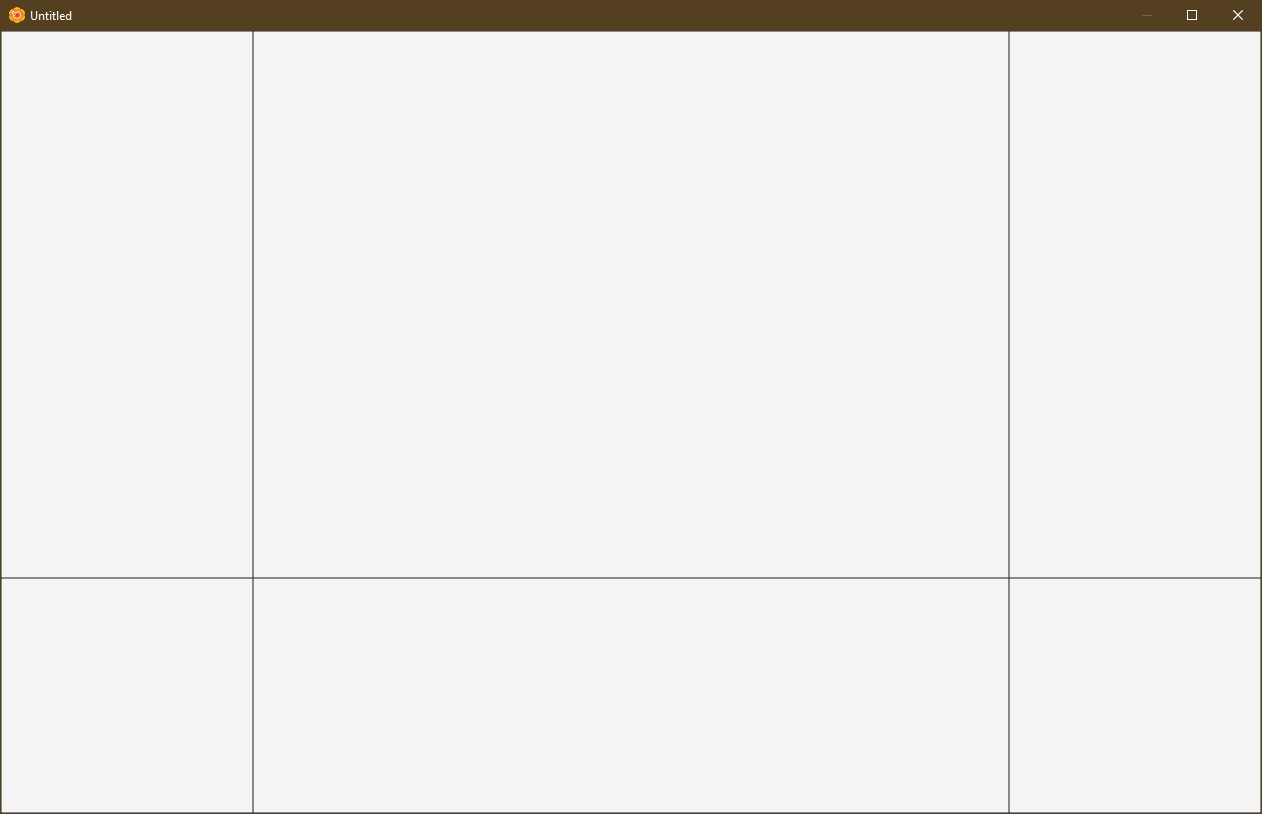
\includegraphics[width=\textwidth]{dissertation/DATA/grid layout.jpg}
    \caption{Grid layout produced from Listing \ref{lst:hardcode_ui}}
    \label{fig:gridss}
\end{figure}

Alternatively, JavaFX \cite{sunmicrosystems_2022_javafx} provides a templating language called FXML and a tool called SceneBuilder \cite{gluon_2022_scene} as discussed in the research section, allowing us to quickly build user interfaces via drag and drop.

Listing \ref{lst:fxml_example} shows part of our FXML code representing the Speed Slider and Clear, Reset and Run Buttons. Directly writing this FXML code is possible but would be very time consuming, and the equivalent Java code would be made up of creating new objects for every capitalised tag (VBox, Pane, ButtonBar, Button, Slider). Instead, by using SceneBuilder \cite{gluon_2022_scene} this section (Figure \ref{fig:fxml_view}) was built within minutes, with the underlying FXML being produce automatically.

\begin{lstlisting}[language=XML,morekeywords={VBox, Pane, ButtonBar, Button, Slider, AnchorPane, Insets}, caption=FXML code to generate the layout in Figure \ref{fig:fxml_view}, label=lst:fxml_example]
<VBox prefHeight="200.0" prefWidth="100.0" AnchorPane.bottomAnchor="0.0" AnchorPane.leftAnchor="0.0" AnchorPane.rightAnchor="0.0" AnchorPane.topAnchor="0.0">
   <children>
      <Pane fx:id="editorPane" prefHeight="778.0" prefWidth="381.0" />
      <ButtonBar prefHeight="40.0" prefWidth="200.0">
        <buttons>
          <Button fx:id="runButton" mnemonicParsing="false" text="Run" ButtonBar.buttonData="RIGHT" />
            <Button fx:id="clearButton" layoutX="412.0" layoutY="18.0" mnemonicParsing="false" text="Clear" ButtonBar.buttonData="LEFT" />
            <Button fx:id="resetButton" layoutX="412.0" layoutY="18.0" mnemonicParsing="false" text="Reset" ButtonBar.buttonData="RIGHT" />

        </buttons>
         <VBox.margin>
            <Insets left="5.0" right="5.0" />
         </VBox.margin>
      </ButtonBar>
      <Slider fx:id="animationSpeedSlider" blockIncrement="1.0" majorTickUnit="2.0" max="10.0" minorTickCount="1" showTickLabels="true" showTickMarks="true" value="1.0" />
   </children>
</VBox>
\end{lstlisting}

\begin{figure}[h]
    \centering
    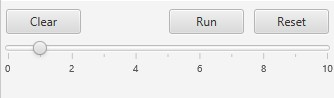
\includegraphics{dissertation/DATA/implemented_slider_run_reset_clear.jpg}
    \caption{Visual render of implemented FXML in Listing \ref{lst:fxml_example}}
    \label{fig:fxml_view}
\end{figure}

As in Figure \ref{fig:fxml_view} the resulting visual layout is quite simple. However, it requires a large quantity of FXML to produce, mainly being all the positional wrapping elements such as AnchorPanes and VBox's. These Anchor panes allow us to anchor edges of elements to the parent causing them to fill the available space. Alternatively, VBox's controlling the flow of elements, with a VBox denoting vertical flow, and a HBox providing a horizontal flow..

\subsubsection{Controllers}\label{sec:impl_emu_controllers}
In order to interact with the FXML elements, JavaFX \cite{sunmicrosystems_2022_javafx} makes us of \texttt{Controller}'s. A controller is a class that contains the logic for interactive \ac{UI} elements.

To connect the FXML elements to our code, JavaFX \cite{sunmicrosystems_2022_javafx} provides the \texttt{@FXML} annotation, which is specified on a variable representing the same element type as the FXML element. For example Listing \ref{lst:fxml_anno} shows how we would obtain a reference to the Run button in Figure \ref{fig:fxml_view}, and then attach a handler it to run code to start the emulation.

\begin{lstlisting}[caption=FXML annotation for a button, label=lst:fxml_anno]
@FXML
private Button runButton;

/*...*/

runButton.setOnAction(e -> {
    resetHandler.run();
    runButton.setDisable(true);
    try {
        Emulator.getInstance().emulate(ca.getText());
    } catch (Exception ex) {
        this.showErrorBoxForException(ex);
    }
});
\end{lstlisting}

In order to allow for this connection the FXML file must be loaded, the controller attached, and the resulting package provided to the stage. The stage is the main \ac{UI} element shown to the user, with all elements being children of the stage. Listing \ref{lst:controller_loader} demonstrates how the application boots the \ac{UI} from setting the window name and position, and loading the controller (\texttt{MainWindowController}) and the FXML file (\texttt{main.fxml}).

\begin{lstlisting}[caption=\ac{UI} starting point, label=lst:controller_loader]
@Override
public void start(Stage stage) throws Exception {
    stage.getIcons().addAll(new Image(VisualStartingPoint.class.getResourceAsStream("/cpu-64x64.png")), new Image(VisualStartingPoint.class.getResourceAsStream("/cpu-32x32.png")));
    VisualStartingPoint.stage = stage;
    stage.setTitle("Visual RISC-V Simulator");

    FXMLLoader loader = new FXMLLoader(getClass().getResource("/main.fxml"));
    MainWindowController mwc = MainWindowController.getInstance();
    loader.setController(mwc);
    Parent croot = loader.load();
    mwc.init(stage);
    Scene sscene = new Scene(croot);
    stage.setScene(sscene);

    stage.setX(0);
    stage.setY(0);
    stage.show();

    Rectangle2D screen = Screen.getPrimary().getBounds();

    stage.setMaxHeight(screen.getHeight());
    stage.setMaxWidth(screen.getWidth());

    ModuleManager.getInstance().start();

    VisualStartingPoint.hostServices = this.getHostServices();
}
\end{lstlisting}

With this the \ac{UI} can be loaded and show to the end user, with all the interactive components linked up to the code for use by the emulator. With the final implemented design in Figure \ref{fig:final_implemented_design} taking into account our design considerations for colourblind users and visual impairments, as well as Nielson's Principles \cite{nielsen_2020_10}.

\begin{figure}[H]
    \centering
    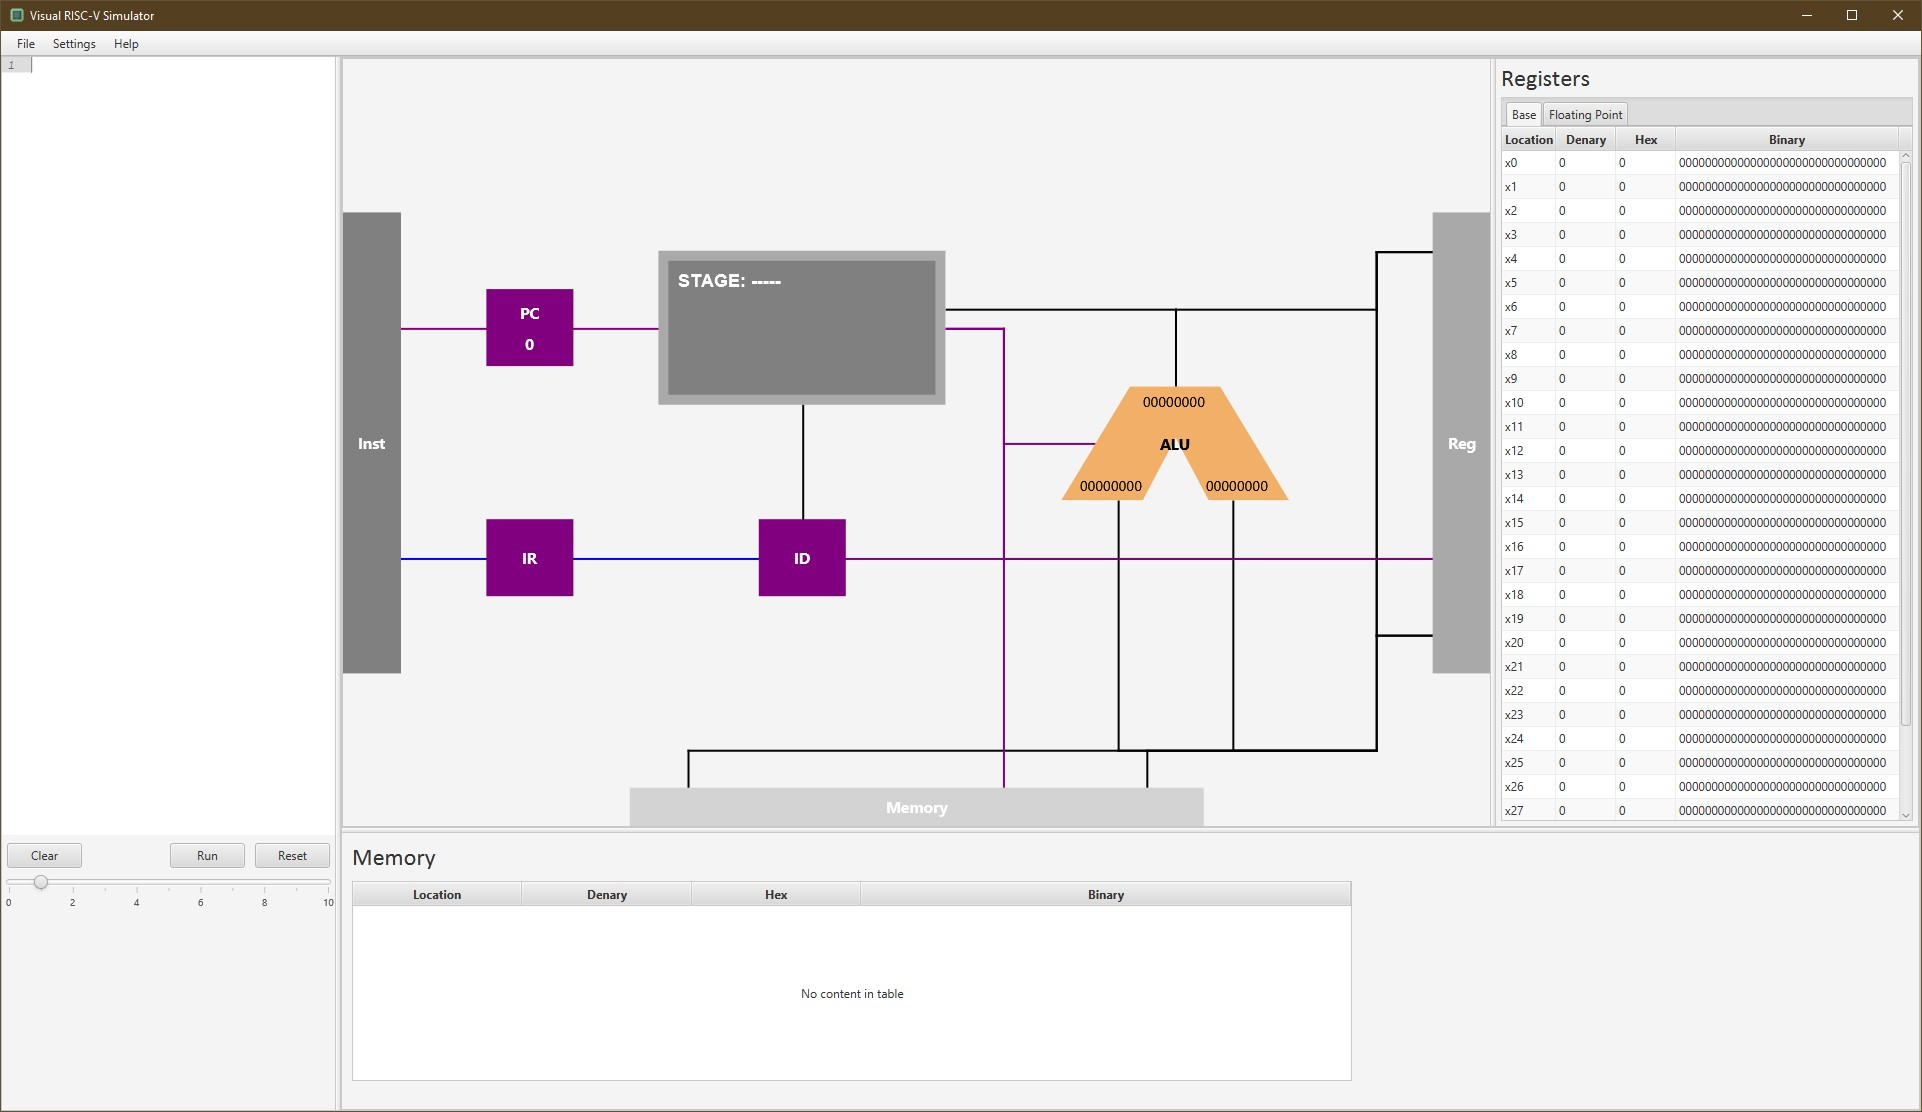
\includegraphics[width=\textwidth]{dissertation/DATA/final_design.jpg}
    \caption{Fully Implemented \ac{UI}}
    \label{fig:full_impl_ui}
\end{figure}

\subsection{Drawing and Animating Paths}\label{sec:paths}
With the \ac{UI} layout implemented, the focus shifted onto producing the animation aspect of the project to allow for the full simulation of instructions.

\subsubsection{Drawing}
JavaFX \cite{sunmicrosystems_2022_javafx} doesn't directly provide a way to produce the kind of paths required for our animation. It does provide a \texttt{Path} class that produces paths. However, it includes functionality that wouldn't be used or required. Thus a custom Path class was produced that tracks a set of points, drawing lines between each set of points using the \texttt{Line} class as seen in Listing \ref{lst:lines}:
\begin{lstlisting}[caption={Example usage of the Line class}, label=lst:lines]
Line line = new Line();
line.setStartX(startX);
line.setStartY(startY);
line.setEndX(endX);
line.setEndY(endY);
\end{lstlisting}

With each point stored in a \texttt{Point} class holding the x and y value of each point. Each path itself is also given a name, this allows us to reference paths later when building up animation sequences, and also helps to identify them during debugging.

In order to simplify the creation of paths, a builder pattern was adopted in the form of a \texttt{PathBuilder} class (Listing \ref{lst:path_builder}), which starts with the Path's name and starting point, and then adding new points to the path, finally building the path once completed returning the newly created \texttt{Path} instance.

\begin{lstlisting}[caption=Path Builder, label=lst:path_builder]
public class PathBuilder {

    private final Path path;

    public PathBuilder(String pathName, double startX, double startY, HBox parent) {
        this.path = new Path(pathName, parent);

        this.path.addPoint(new PathPoint(0,0)); // We have to build a fake first path to get it to position correctly
        this.path.addPoint(new PathPoint(startX, startY));
    }

    public PathBuilder addPoint(double x, double y) {
        this.path.addPoint(new PathPoint(x, y));
        return this;
    }
    
    public Path build() {
        PathRegister.getInstance().register(this.path);
        return this.path;
    }
}
\end{lstlisting}

Due to the nature of building these paths and having them position correctly on screen, an additional invisible line has to be drawn for every path as seen in Listing \ref{lst:path_builder} on line 8. This was due to the fact that JavaFX \cite{sunmicrosystems_2022_javafx} defines (0,0) based on the first added line. Thus if a invisible line wasn't drawn, a line starting at 100,100 would appear in the very top left of the parent, instead of being at (100,100) as expected. Hence, drawing an invisible line first from 0,0 to our starting point alleviates this issue without impacting the visualisation.

With the builder created we can use it to produce all the paths as seen in Figure \ref{fig:final_implemented_design}, with the following code used to produce the line connecting the \ac{IR} and \ac{ID} as seen in Listing \ref{lst:path_builder}:
\begin{lstlisting}[caption=Example of use the path builder, label=lst:path_builder]
(new PercentagePathBuilder("IR_TO_ID", 20, 65, anim)).addPoint(36.25, 65).build().autoDraw(animationGroup, blue);
\end{lstlisting}

\subsubsection{Animating}
With our ability to draw paths, we now need to be able to animate on top of the to show the flow of data. JavaFX \cite{sunmicrosystems_2022_javafx} provides a few transition methods, with the main two being \texttt{TranslateTransition} and \texttt{SequentialTransition}, which allows us to translate elements, and sequentially run transitions respectively.

The logic for the animating over a specific path is contained within the \texttt{Path} class. Much like for drawing paths, we loop over all of the paths points, this time creating a new \texttt{TranslateTransition} for each pair of points. The transition is told to translate the given data element by the difference between the coordinates, and to animate this in a linear fashion as seen is Listing \ref{lst:translate}.

\begin{lstlisting}[caption=Translate Transition for two points, label=lst:translate]
TranslateTransition tt = new TranslateTransition();

/*...*/

tx =  (next.getX() * parentWidth - point.getX() * parentWidth);
ty =  (next.getY() * parentHeight - point.getY() * parentHeight);

tt.setByX(tx);
tt.setByY(ty);
tt.setInterpolator(Interpolator.LINEAR);
\end{lstlisting}

Due to the transition between each set of point varying in distance, the duration needed to be modified to ensure that the moving data element crossed each path at the same speed, instead of crossing each at different speeds. This was fixed by specifying a fixed speed for all animations of 100 pixels/second. Then by using the simple formula of $time = distance/speed$ the respective transition time could be calculated to ensure a constant speed over all paths.

Then each \texttt{TranslateTransition} could be added to the main \texttt{SequentialTransition}. Then when played, each \texttt{TranslateTransition} is played one after the other until all of them have played, or the animation is cancelled by the user.

In order to allow for speed control as specified in requirement \ref{req:speed}, we can adjust the rate at which the \texttt{SequentialTransition} plays by binding the value of the slider to the rate property as seen in Listing \ref{lst:slider}:
\begin{lstlisting}[caption=Slider linking code, label=lst:slider]
SequentialTransition sq = new SequentialTransition(circle);
sq.rateProperty().bind(MainWindowController.getInstance() .getAnimationSpeedSlider().valueProperty());
\end{lstlisting}
With a value between 0 - 10 allowing for pausing at 0, to a very fast animation with a value of 10.

With the ability to now animate over individual paths, a way to animate over multiple paths, as well as provide other actions need to be produces.

A custom class called \texttt{Animator} (Listing \ref{lst:anim_stage}) handles this for us. Again it follows a builder pattern to build up animations, with each section being denoted as a \texttt{AnimatorStage}, which is an abstract class, providing a \verb|play()| method to be implemented for the respective stage, as well as providing a convenient \verb|next()| method to call the next stage from within each stage.

\begin{lstlisting}[caption=Abstract \texttt{AnimatorStage} class, label=lst:anim_stage]
public abstract class AnimatorStage {
    protected Animator animator;

    public AnimatorStage(Animator animator) {

        this.animator = animator;
    }
    public abstract void play(StackPane circle);

    public void setAnimator(Animator animator) {
        this.animator = animator;
    }

    /**
     * Will run once he stage has finished, cleaning up itself and then calling animator.next()
     */
    public void after() {
        animator.next();
    };

}
\end{lstlisting}

The main stage is the \texttt{PathStage} which is provided with a path instance, and then runs the provided paths animation when the stage is run. The following stages also exists:

\begin{itemize}
    \item \texttt{RunStage} - Permits the running of any arbitrary code when the stage is executed,
    \item \texttt{InterpolateToPathStage} - Translates the visual data element between its current position and the start of the next path smoothly,
    \item \texttt{ALUStage} - Updates the visual elements of the\ac{ALU},
    \item \texttt{MemoryStage} - Updates the memory table,
    \item \texttt{TextChangeStage} - Updates the text on the visual data element.
\end{itemize}

Each of these stages can then be individually added via the \texttt{Animator} builder. The \texttt{Animator} then provides \verb|start()| and \verb|stop()| functions, as well as automatically registering all to a static list, to allow for the stopping of all animations at the same time, as the system supports parallel running of multiple animations at once.

For example we can use the code in Listing \ref{lst:animator_follow} to animate between the \ac{IR} and \ac{ID}:
\begin{lstlisting}[caption=Example of animating with the Animator, label=lst:animator_follow]
Animator().setText("I").followPath("IR_TO_ID").setText("D") .setText("D").followPath("ID_TO_CU");
\end{lstlisting}

\subsubsection{Fixed Elements}
Within the animation area in the centre of the screen, other than drawing path there are also fixed boxes to represent various components. 

These are then drawn to screen using the \texttt{VBox} element with a coloured background and then text on top. Each element exists as an extension of a abstract \texttt{VisualItem} class. This class does the heavy work of positioning the element on screen, as well as creating the default box structure with the text centred inside, as these are defined purely in code  and not with FXML. The class provides an abstract \verb|decorate()| method that allows each element to add additional styling or completely override the base styling.

For example the \ac{CU} overrides the base implementation to allow it to display more text to keep the user updated on what the system is doing, with a base method called \verb|updateCUContent| to specify the \ac{CU} content, with 5 methods sitting on top specifying the contents for the Fetch, Decode, Execute, Memory and Write cycle. (See Listing \ref{lst:cu_comp}).

\begin{lstlisting}[caption={\ac{CU} content updater methods}, label={lst:cu_comp}]
public void showFetch(ExecutableInstruction executableInstruction, int instructionMemLoc) {
    this.updateCUContent("fetch", executableInstruction, "READ", "LOC: " + instructionMemLoc);
}

/* ... showDecode, showExecute, showMemeory and showWrite ... */

private void updateCUContent(String stageName, ExecutableInstruction ei, String... options) {
    this.stageText.setText("STAGE: " + stageName.toUpperCase());
    this.options.getChildren().clear();
    this.options.getChildren().add(ComponentFactory.classText(ei.getInstruction() .getIdentifier() + " " + String.join(", ", ei.getOperands().getOperands()), "cu-option"));
    for (String option : options) {
        this.options.getChildren().add(ComponentFactory.classText(option, "cu-option"));
    }
}
\end{lstlisting}

\subsection{Callbacks and CompletableFutures}\label{sec:call_vs_cf}
Within the \texttt{Animator} we make heavy use of callbacks to control the flow of animations, with the end of one stage, calling for the next to be played, and so on. This is permitted via the \texttt{AnimatorFinishedCallback} interface, which simply allows us to encapsulate logic to be execute later. Alongside the callback functions of the \texttt{SequentialTransition} the whole animation sequence is played out.

Whilst this system works, it is prone to a issue of having to nest callbacks in places. For example in the code to run the 5 animation sections discussed in the Integration Section \ref{sec:impl_integ}, the following code is used to control the conditional execution of instructions with no \verb|execute()| handler as seen in Listing \ref{lst:cond_call}
\begin{lstlisting}[caption=Conditional callback execution, label=lst:cond_call]
decode.onFinish(() -> {
    if (execute != null) {
        ControlUnit.getInstance().showExecute(this, ProgramCounter.getProgramCounter().getValueAsInteger());
        execute.onFinish(() -> {
            ControlUnit.getInstance().showMemory(this);
            memory.start();
        });
        execute.start();
    } else {
        ControlUnit.getInstance().showMemory(this);
        memory.start();
    }
});
\end{lstlisting}
It contains a \verb|onFinish| call within another, which works, but isn't the nicest to write, and can become far more complex if more intricate animation sequences are needed.

A solution to this would be to make use of \texttt{CompletableFuture}'s. These allow us to wrap the callback operation into a more functional approach in which our code will wait for the async operation to complete before executing the next line, instead of specifying a callback to be executed later. 

The above callback code could be written as seen in Listing \ref{lst:pseduo} (pseudo code).
\begin{lstlisting}[caption=Functional pseduo code, label=lst:pseduo]
decode.start();
if (execute != null) execute.start()
memory.start()
\end{lstlisting}
This allows for the code to block until the current animation has finished and then moving onto the next line. This means no callback functions or async execution. This massively reduces the complexity of writing code to control the animation flow. On the other hand, it does require more additional design and setup to implement the \texttt{CompletableFuture} classes.

Listing \ref{lst:complt_future} shows an example of a \texttt{CompletableFuture} that just waits for 1 second before returning.

\begin{lstlisting}[caption=Example completable future code from CalliCoder.com \cite{singh_2022_java}, label=lst:complt_future]
CompletableFuture<Void> future = CompletableFuture.runAsync(new Runnable() {
    @Override
    public void run() {
        // Simulate a long-running Job
        try {
            TimeUnit.SECONDS.sleep(1);
        } catch (InterruptedException e) {
            throw new IllegalStateException(e);
        }
        System.out.println("I'll run in a separate thread than the main thread.");
    }
});

// Block and wait for the future to complete
future.get()
\end{lstlisting}

Currently the project doesn't make use of \texttt{CompletableFuture}'s, and this is something that will be refactored in in the future as it will require major breaking changes to the project code to implement.

\subsection{Percentages over Coordinates}
Within the implementation of paths an animations, path points were being stored as physical coordinates. Whilst this worked, it proved difficult to manually position the paths and box elements on screen. Coordinates had to be produces as a result of trial and error to position them perfectly. With this becoming much harder for ensuring paths overlaid on top of each other when they joined up, without producing a double thick path due to incorrect coordinates.

The intuitive solution was to switch to percentages. With percentages, each point was defined as a percentage of the width and height of the parent element, with (0\%,0\%) being in the top-left and (100\%,100\%) being in the bottom-right of the parent. This immediately made positioning paths and elements much quicker and easier, avoiding having to manually calculate element positions, leaving the application to automatically calculate these positions during run time.

Further this also allowed the \ac{UI} to be resizable instead of a fixed size. Originally, because of the fixed coordinate points, the animation area would remain a fixed size whilst the result of the \ac{UI} scaled as the user resized the application window, an original fix was to scale the parents contents, however this produced odd results with lines and elements colliding and not resizing correctly. However, when using percentages, the new positions of elements and lines can be recalculated based on the parent by simply multiplying the width/height by the percentage.

In order to implement this, the pathing classes had to be completely rewritten to support percentages. This mainly consisted of switching out the logic for calculating positions of points, from a fixed value, to a dynamically calculated value based on the parent as seen in Listing \ref{lst:perc_points}.
\begin{lstlisting}[caption=Percentage point caculations, label=lst:perc_points]
point.getX() * parentWidth

// Distance between current and next point:
tx = (next.getX() * parentWidth - point.getX() * parentWidth);
ty = (next.getY() * parentHeight - point.getY() * parentHeight);
\end{lstlisting}

To permit dynamic resizing, a resize listener was created to check for window resizes, and then call for the entire animation area to be redrawn instantly. This also called for any active animations to be hidden, and a new animation started at the new resized values, with the old animations being removed after. Due to the design of the animation system we can't simply reuse the active animation, as it pre-computes the values for each stage of the animation based on the current window size, and thus it would result in the animated element clipping through the resized elements, leaving paths of going off screen.

\begin{lstlisting}[caption=Auto draw function, label=lst:auto_draw]
public void autoDraw(Group drawGroup, Color clr) {
    this.parent.widthProperty().addListener((obs, oldV, newV) -> {

        removeLines(drawGroup);
        draw(drawGroup, clr);
        updateInprogressTransitionOnWindowResize();
    });
    this.parent.heightProperty().addListener((obs, oldV, newV) -> {

        removeLines(drawGroup);
        draw(drawGroup, clr);
        updateInprogressTransitionOnWindowResize();
    });
}
\end{lstlisting}

This is all handled by the \verb|autodraw()| function in Listing \ref{lst:auto_draw} and the \\ \verb|updateInprogressTransitionOnWindowResize()| function in Listing \ref{lst:resize_anim}.

\begin{lstlisting}[caption=Function to update inprogress animations on a window resize, label=lst:resize_anim]
private void updateInprogressTransitionOnWindowResize() {

    List<ActiveAnimation> toRestart = new ArrayList<>();
    toRestart.addAll(activeAnimations);

    for (ActiveAnimation activeAnimation : activeAnimations) {
        activeAnimation.getSequentialTransition().pause();
        activeAnimation.getSequentialTransition().setOnFinished(null);
        //activeAnimation.getSequentialTransition().stop();

    }

    activeAnimations.clear();

    toRestart.forEach(activeAnimation -> {
        StackPane activeCircle = activeAnimation.getCircle();
        EventHandler eventHandler = activeAnimation.getEventHandler();

        this.animate(activeCircle, eventHandler, activeAnimation.getSequentialTransition().getCurrentTime());
        activeAnimation.getSequentialTransition().stop();
        activeCircle.toFront();
    });

    toRestart.clear();
}
\end{lstlisting}

The automatic replaying of resized animations in significantly more complex than just re-drawing the lines and elements. This is due to needing to track all the active animations and their progress. Thankfully the \texttt{SequentialTransition} class tracks its progress through all the transitions and allows us to start the transition at any given point. 

Combined with simply tracking any currently active animation by individually tracking them in each \texttt{Path} class, the auto resizing can automatically stop any active animations and then immediately start new animations based on the newly resized windows, copying over the resulting callback functions and starting at the exact position the previous animation stopped for a very smooth experience with no tearing or odd behaviour.

In order to track an active animation, when a new animation is played a \texttt{ActiveAnimation} instance is created (Listing \ref{lst:active_anim}) which acts as a wrapper containing a reference to its parent \texttt{SequentialTransition}, the active animation element (referred to as the \texttt{circle}) and its callback event handler. It is then appended to a list of active animations that can be iterated through on a window resize to cause the animation resizing as discussed in the paragraph above.

\begin{lstlisting}[caption=ActiveAnimation wrapper, label=lst:active_anim]
class ActiveAnimation {
    private final SequentialTransition sequentialTransition;
    private final StackPane circle;
    private final EventHandler eventHandler;
    
    public ActiveAnimation(SequentialTransition sequentialTransition, StackPane circle, EventHandler eventHandler) {
        this.sequentialTransition = sequentialTransition;
        this.circle = circle;
        this.eventHandler = eventHandler;
    }
    
    public SequentialTransition getSequentialTransition() {
        return sequentialTransition;
    }
    
    public StackPane getCircle() {
        return circle;
    }
    
    public EventHandler getEventHandler() {
        return eventHandler;
    }
}
\end{lstlisting}


\section{Integration}\label{sec:impl_integ}
With the Emulator (Section \ref{sec:impl_emul}) and Visualisation (Section \ref{sec:impl_vis}) created, they need to be combined to work together in a tight integration. In the previous Visualisation section \ref{sec:impl_vis} various code listing hinted to this integration, mainly via the use of linking the visual \ac{UI} elements to the emulator code via the \texttt{@FXML} annotation and controllers \ref{sec:impl_emu_controllers}.

Our controllers exist in a hierarchy of the main \texttt{MainWindowController} starting by loading all the FXML annotations, and passing them to numerous sub-controllers that each handle the functionality of sections of the \ac{UI}. As a result there are 4 sub-controllers:
\begin{itemize}
    \item \texttt{VisualPaneController} - Handles management of all the path builders, and animated area,
    \item \texttt{CodeEditorController} - Handles the physical code editor and its functionality, as well as the buttons and slider below,
    \item \texttt{RegisterController} - Handles managing the register table and refreshing it,
    \item \texttt{MemoryController} - Handles managing the memory table and refreshing it,
    \item \texttt{SettingsController} - Handles loading and showing the settings pane,
    \item \texttt{AboutController} - Handles loading and showing the settings pane,
\end{itemize}

In the next 5 sub-sections, the modifications made to the emulator and visualisation to produce the tight integration are discussed, along with fixing a specific issue with register updating in sub-section \ref{sec:early_update_prob}.

\subsection{The 5 Animation Stages}
In order to provide a suitable animation sequence that is triggered by the emulation, it was decided that each instructions animation would be split into the 5 respective parts of the Fetch, Decode, Execute, Memory and Write cycle. This deviates from normal with most processors having 3 stages. RISC-V has 5 stages as RISC-V instructions are very simple and can be more easily pipe-lined in parallel with 5 stages. This way, common animations such as the fetching of an instruction from the instruction memory to the \ac{CU} could be written once, and then overridden if needed. This was permitted by amending the abstract \texttt{Instruction} class to include Fetch, Decode, Memory and Write methods along side the existing Execute method, as seen in Listing \ref{lst:fdemw}.

\begin{lstlisting}[caption={Additional Fetch, Decode, Memeory and Write methods added to the abstract \texttt{Instruction } class}, label=lst:fdemw]
public Animator fetch() {
    return new Animator() .setText(ProgramCounter.getProgramCounter().getValueAsHex()) .followPath("PC_TO_INSTR").setText("I").setText("I") .followPath("INSTR_TO_IR");
}

public Animator decode() {
    return new Animator() .setText("I").followPath("IR_TO_ID").setText("D").setText("D") .followPath("ID_TO_CU");
}

public Animator memory() {
    return new Animator();
}

public Animator write() {
    return new Animator();
}
\end{lstlisting}

With these additional stages, any individually instruction can override any of the animations as required, or extend them to include extra details or disable them entirely. These can then be executed linearly as seen in Listing \ref{lst:complt_future} in Section \ref{sec:call_vs_cf} via callbacks.

For more sophisticated animations and similar instructions, boilerplate code was refactored out into super-classes representing these similar instructions. For example the abstract \texttt{ALUCommonInstruction} class encapsulates the logic for instructions that take two registers and perform an arithmetic operation on them, providing a \verb|calc(int rs1, int rs2)| method than can be overridden by individual sub-classes such as the instruction class for \texttt{ADD} which can be seen in Listing \ref{lst:add_subclass}.

\begin{lstlisting}[caption={ADD Insutrction, making useof the \texttt{ALUCommonInstruction} class}, label=lst:add_subclass]
public class ADD extends ALUCommonInstruction {
    public ADD() {
        super("ADD");
    }

    @Override
    public int calc(int rs1, int rs2) {
        return rs1 + rs2;
    }

    @Override
    public String operator() {
        return "+";
    }
}
\end{lstlisting}

Further, the animations can also be abstracted away for these common instruction types. By abstracting this code out it become much more maintainable and follows the DRY (Don't Repeat Yourself) principle, with the code existing once, allowing for changes to reflect globally, instead of having to make the same change numerous times in different files.

This resulted in the creation of the \texttt{ALUAnimationBuilder} class.  This class provides a quick way to specify the animation for an arithmetic operation on tow register values, supplying the operator, registers and output. Internally it manages the creation of the required \texttt{Animators} to allow for an animation of data flowing into the \ac{ALU} from the registers and then the operation being applied, before finally sending it back to the registers. The builder provides two functions \verb|buildExecute()| and \verb|buildWrite| which return the respective \texttt{Animators} for the Execute and Write animation sequence. 

On top of the \texttt{ALUAnimationBuilder}, there is also a \texttt{CommonAnimationsFactory} class which provides quick access to an instance of the \texttt{ALUAnimationBuilder}, as well as static methods to provide quick generation of common animations such as moving data between the registers and \ac{ALU} and sending signals to various components, allowing much faster building of animation sequences instead of having to manually write the same lines over and over again, as seen in Listing \ref{lst:dry}

\begin{lstlisting}[caption=Factory method building a more complex animation moving data from the registers to the \ac{ALU},label=lst:dry]
public static Animator regToALU(Animator animator, Binary value, ALUConnection conn, boolean interp) {
    animator.setText(value.getValueAsHex()).followPath("REG_OUT");

    if (interp) {
        animator.interpolateAndFollowPath("REG_OUT_TO_RM-JUNCTION");
    } else {
        animator.followPath("REG_OUT_TO_RM-JUNCTION");
    }

    if (conn == ALUConnection.IN_1) {
        animator.followPath("ALU_IN_1");
    } else {
        animator.followPath("ALU_IN_2");
    }

    return animator;
}
\end{lstlisting}

\subsection{Memory and Registers}
The registers and memory both require a suitable representation on screen, with a table being the most ideal. Currently both register and memory values are just simply dumped as text onto the screen. Thankfully JavaFX \cite{sunmicrosystems_2022_javafx} provides a element called \texttt{TableView} which allows us to generate tables and fill them with data that can be updated in real time.

For both the registers and memory the tables being as an FXML element with the 4 columns (Register/Location, Denary, Hex and Binary) already pre-set, but with no data. Within the \texttt{RegisterController} and \texttt{MemoryController} references are obtained to both the table element and each individual column. With this we can specify a value factory for each column, these value factory will automatically pull a value from the passed class. They do this by us specifying the name of the function that returns each respective value, omitting "get" from them, in this case we can see in Listing \ref{lst:table_view} that for the location, denary, hex and binary we specify the respective function name on the \texttt{Register} class. Now when passing a list of \texttt{Register}'s from the \texttt{RegisterSet} instance, the table will automatically fill each row with the required data.

\begin{lstlisting}[caption=\texttt{RegisterController} code to obtain column values, label=lst:table_view]
location.setCellValueFactory(new PropertyValueFactory<>("Name")); // will call Register#getName()
denary.setCellValueFactory(new PropertyValueFactory<>("ValueAsInteger")); // will call Register#getValueAsInteger()
hex.setCellValueFactory(new PropertyValueFactory<>("ValueAsHex")); // will call Register#getValueAsHex()
binary.setCellValueFactory(new PropertyValueFactory<>("Value")); // will call Register#getValue()
\end{lstlisting}

The memory operates the same for attaching column values, however both controllers make use of slightly different mechanisms to refresh the table data. The register table always maintains a list of the 32 base register, calling for the register values to be re-fetched on refresh. On the other hand due to memory's dynamic nature, each refresh makes a call to the \texttt{Memory} instance, to obtain a fresh list of any available memory cells, automatically sorting them via the location in an ascending nature.

\subsubsection{The Early Update Problem}\label{sec:early_update_prob}
The table views work exceptionally well with no issues themselves. However, during testing a problem in which when writing to a register, the value in the table would update before the write animation had finished. This caused some confusion as it implied that any register changes are written instantly, which may seem the case in the real world, but there will be a small quantity of time of which the data is travelling, which the simulator should also display.

The root of the problem was due to the writing of register values being separate to the animation sequence. Register values are set via a \verb|write| class on the \texttt{RegisterSet} class. However, this executes instantly which originally wasn't considered an issue with registers updating once each instruction has finished executing. Unfortunately, due to the callback nature, this refreshing was often called mid way through execution resulting in the emulation being one induction ahead of the visualisation, resulting in register updating before the animation had ended.

Two fixes were identified, the first including moving register writing into a animation stage, however this proved to be tricky to implement and didn't work consistently enough to be viable. The second was to buffer register writes, and make use of an animation stage to then flush them through the system calling a refresh after. This worked perfectly, with only minor changes required to the \texttt{RegisterSet} class as seen in Listing \ref{lst:reg_buffer}. These included: 
\begin{itemize}
    \item Adding a set to act as a buffer of changes (this won't cause missed writes, as it is flushed per instruction),
    \item Modifying the write to push writes to the buffer instead of immediately writing to the registers,
    \item Adding a \textbf{refresh()} function, that iterates over the write buffer, writing the changes to the respective registers.
\end{itemize}

\begin{lstlisting}[caption={Refresh mechanism, writing buffered register values}, label=lst:reg_buffer]
private final Set<Register> toUpdate;

public void write(String registerName, String value) throws RegisterNotFoundException, InvalidValueException {
    if (ignoreZeroRegister(registerName)) return;

    // Check the given value is infact binary
    Utils.isBinary(value); // throws its own error

    Register cloned = this.load(registerName).clone();

    cloned.setValue(value);

    this.toUpdate.add(cloned);
}
    
public void refresh() {
    toUpdate.forEach(reg -> {
        this.registerMap.get(reg.getName()).setValue(reg.getBinary());
    });
    toUpdate.clear();
}
\end{lstlisting}

\subsection{Pushing updates}
Within some of the visual animation components, it was imperative that their text updated during animations. This required a way to push updated information to them. A common way to create this functionality is creating an even/bind. For the project, a generic \texttt{Bind} interface was created which simply provides a \verb|execute(E value)| method. Generics have been made us of here so that a bind may update any kind of value. 

A bind is created by simply creating a new instance of a bind and implementing the \verb|execute(...)| method. It can then be called by running \verb|bind.execute(...)|. This allowed for the simple updating of the \ac{ALU} text with Listing \ref{lst:bind} showing how the a bind is created to provide a \texttt{Binary} instance and set the respective text value as well as how the \texttt{ALUStage} calls the bind with a \texttt{Binary} instance.

\begin{lstlisting}[caption=\ac{ALU} bind creation and execution, label=lst:bind]
this.inBind1 = (binary) -> {in1.defaultText.setText(binary.getValueAsHex());};
this.inBind2 = (binary) -> {in2.defaultText.setText(binary.getValueAsHex());};
this.outBind = (binary) -> {out.defaultText.setText(binary.getValueAsHex());};

...

ALU alu = ALU.getInstance();
alu.getInBind1().execute(this.in1); 
alu.getInBind2().execute(this.in2);
\end{lstlisting}

Thanks, to this simple interface it makes pushing data relatively simple, and due to the generic nature we could of also specified the bind take a string value, an integer or even a \texttt{Register} instance itself.

\subsection{Code Editor}
After creating the visualisation, the method of inputting RISC-V assembly was rather basic, with just a simple text box. It would be more intuitive and friendly for the code editor to have similar features to other simulators and some integrated development environments. Including basic syntax highlighting and line numbers to make debugging easier.

JavaFX \cite{sunmicrosystems_2022_javafx} has a convenient library called RichTextFX \cite{fxmisc_2023_fxmiscrichtextfx}, which provides a \texttt{CodeArea} class which allows us to produce a customised code editor with support for syntax highlighting and line numbers.

To allow for syntax highlighting RichTextFX \cite{fxmisc_2023_fxmiscrichtextfx} requires us to compute and apply styled spans which apply a set of styles to a specific area of text based on the index of the first character and the length.

These spans are computed using regex. First a pattern is compiled that recognises all the loaded instruction names and any comments (starting with a \%). It is then matched against the entered code, with the start and length of each match being stored alongside the respective style class to be applied. These are then returned to the \texttt{CodeArea} instance, that applies the spans resulting in the styling appearing.

Styles in this case mimic web-based Cascading Style Sheets, with a class encapsulating styling properties, that are applied to each matched element. In this case we have the \verb|.instr| and \verb|.comment| classes which make instruction names purple and bold, and comments green alike as seen in Figure \ref{fig:syntax_high}.

\begin{figure}
    \centering
    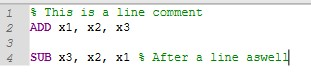
\includegraphics[width=0.6\textwidth]{dissertation/DATA/syntax_high.jpg}
    \caption{Example of applied syntax highlighting}
    \label{fig:syntax_high}
\end{figure}


\section{Module System}\label{sec:impl_mod}
Later in development, when the stage of implementing additional RISC-V \cite{fxmisc_2023_fxmiscrichtextfx} extensions was reached, a modular approach was decided upon as stated in the Design in Section \ref{sec:module}.

To re-iterate from the start of this section: We refer to modules as the encapsulation of logic that allows us to implement a RISC-V extension such as Multiply and Divide.

Modules exist as a implementation of the \texttt{VRVSModule} interface in Listing \ref{lst:vrvs_interface}. Every created module must have their main class implement the 3 provided methods, to allow for the main application to identify each module, and also enable/disable it.

\begin{lstlisting}[caption=\texttt{VRVSModule} interface for creating new modules]
public interface VRVSModule {
    String getName();

    void onEnable(VRVSApi api);

    void onDisable(VRVSApi api);
}
\end{lstlisting}

In the \verb|onEnable(...)| and \verb|onDisable(...)| methods a instance of \texttt{VRVSApi} is provided. This instance provides methods to allow modules to extend the base system, providing a method to add new instructions, add additional code examples and even add additional register panes so that more registers other than the base 32 registers can be seen.

Each \texttt{VRVSApi} instance is specific to a module. This was done to enable the tracking of which module added features via the API, meaning those additions can easily be unloaded by removing all features tagged against the module being disabled. This is done by allocating multiple sets which store references to the added items. These sets can then be iterated over in order to remove all the added items. A set is used here to remove the possibility to adding duplicate items, as a set doesn't permit duplicates, thus if a user were to register the same instruction twice, it wouldn't then attempt to remove it twice, as the internal instruction manager will reject duplicate instructions anyway.

\subsection{Loading Modules}
In order to allow for modules to be loaded, the Java \texttt{ServiceLoader} is used. The \texttt{ServiceLoader} allows us to dynamically load external classes in to the Java Virtual Machine at run time. The loader first requires a set of URL's to load from, in this case we can provide the URL to the module's compile jar file which for example might be called \texttt{Module.jar}. We pass this URL to the \texttt{ServiceLoader}, specifying the class to be loaded. In this case the target class is \texttt{VRVSModule}. As a result, any class implementing \texttt{VRVSModule} will be loaded from the Jar, or list of Jar's given.

These loaded classes are then iterated over and wrapped in a \texttt{LoadedModule} instance, and then finally are checked to see if the user has specified if the respective module is enabled or not, defaulting to being enabled.

However, because of using the \texttt{ServiceLoader} each module is considered a service, and must contain a service identifier that is used to pull the required \texttt{VRVSModule} class. Within the resources section of a modules project, a directory structure of \verb|META-INF.services| must be created, with a file inside with the name of the full \texttt{VRVSModule} class path within the main application, and then each line inside containing the full class path of the modules class implementing the \texttt{VRVSModule} class.

The \texttt{LoadedModule} wrapper exist to provide extra functionality to handling modules that can't be directly inside the module class itself, otherwise it would open it up to modification by module creators. The wrapper provides methods to call the modules enable and disable methods, passing in the modules specific instance of the \texttt{VRVSApi} which is stored inside the \texttt{LoadedModule} wrapper. The wrapper also provides a method to check if a module is enabled, and also allow us to specify if a module is built-in and packaged with the core application, and if so, that this module cannot be deleted, only disabled.

All of these \texttt{LoadedModule}'s are managed by a \texttt{ModuleManager} instance, which holds a reference to every module, and provides functions to load internal and external modules, delete modules and ensure that the required directory structure exists for storing modules. It further provides a simple way to initiate the module system by simply instantiating the \texttt{ModuleManager} class and calling \verb|start()|, and then completely cleaning up on application close by calling \verb|end()|.

\subsection{\ac{UI} Additions}
Currently modules can only be added or removed by manually placing them into the created modules folder on a users system. Thus a easier way to manage modules via the application was implemented through the use of a popup window.

As based on its design the window contains a table listing the loaded modules, and if they are enabled or not, with buttons below to add and delete modules, which can be seen in Figure \ref{fig:module_popup}.

\begin{figure}[H]
    \centering
    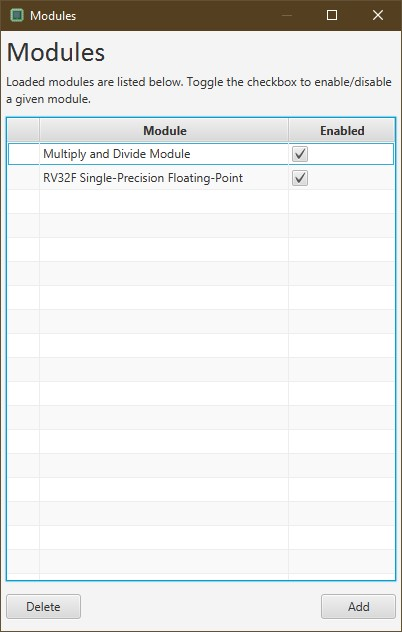
\includegraphics[width=0.5\textwidth]{dissertation/DATA/module_popup.jpg}
    \caption{Implemented Module Popup}
    \label{fig:module_popup}
\end{figure}

The popup is designed using FXML residing in the \texttt{modules.fxml} file, with interactivity added via the \texttt{NewModulePopup} controller. Each row of the table contains the modules name and a checkbox to enable and disable the module. On toggling a module a popup is show to confirm the actions completion.

Additionally, the very first column of the table has he option to display a checkbox for externally added modules. This permit the user o select one or more modules and then click delete. This will ask the user to confirm their decision before the module system unloads and deletes the specified modules.

\section{Additional Features}
\subsection{File Saving/Loading}
The majority of code emulators and simulators permit the saving and loading of user written code, and so shall the project.

This can be quickly implemented by adding menu-bar options to load and save a file, and then implementing the feature inside the \texttt{CodeEditorController} class.

For both loading and saving we make use of the Operating Systems file chooser, via JavaFX's \cite{sunmicrosystems_2022_javafx} wrapper. This wrapper is known as \texttt{FileChooser} and it allows us to specify the default file extension to use as well as open two individual dialogues to allow for retrieving a file and saving a file.

The open dialog returns a \texttt{File} instance, that can be read using builtin file utilise, with its contents being pasted directly into the code editor. For saving, the dialog returns a \texttt{File} instance representing the saved location on the system. Then using a \texttt{PrintWriter} the contents of the code editor an be written to the file and saved as seen in Listing \ref{lst:file_save}.

\begin{lstlisting}[caption=File saving implementation using \texttt{FileChooser}, label=lst:file_save]
FileChooser fileChooser = new FileChooser();
fileChooser.getExtensionFilters().add(new FileChooser.ExtensionFilter("RISC-V", "*.riscv"));

fileSave.setOnAction(e -> {
    fileChooser.setTitle("Save");
    File file = fileChooser.showSaveDialog(VisualStartingPoint.getStage());
    if (file == null) return;
    PrintWriter writer = null;
    try {
        writer = new PrintWriter(file);
        writer.print(ca.getText());
        writer.close();
    } catch (FileNotFoundException ex) {
        new Alert(Alert.AlertType.ERROR, "Failed to save to file!").showAndWait();
    }
});
\end{lstlisting}

\subsection{Animation Toggling}
In some cases a user may not want to simulate their code, and instead just emulate it jumping straight to the end results. To allow for this a toggle was implemented which disables the execution of animations.

This required slight modification to aspects of the emulation code, mainly by passing in the animations toggle into the \texttt{Program} instance, which in turn passes it to each \texttt{ExecutableInstruction} instance. Then when each \texttt{ExecutableInstruction} is executed, if animations are disabled it will only call the referenced instructions \verb|execute(...)| method, ignoring the fetch, decode, memory and write animations. Immediately calling for the execution of the next instruction, ignoring the returned Animator from the \verb|execute()| method as well.

Due to changes to fix the early register updating problem, a check also had to be added here to override this fix for disabled animations, otherwise register writes would never hit the actual registers, causing all operations to result in 0. This modification can be seen in Listing \ref{lst:noAnimModifi}.

\begin{lstlisting}[caption={Modification to register \texttt{write(...)} for instance writing when animations are disabled}, label=lst:noAnimModifi]
if (!SettingsController.areAnimationsEnabled()) {
    Register reg = this.load(registerName);
    reg.setValue(value);
    return;
}
\end{lstlisting}

Once the entire execution is completed, the registers are manually updated by the emulator to show the end results.
